% ============================================================
% 语义回响：通过回收被丢弃Token嵌入增强语言模型表达能力
% Semantic Echo: Enhancing LLM Expressiveness by Recycling Discarded Token Embeddings
% ============================================================

\documentclass[twocolumn, a4paper, 10pt]{article}

% ---------- 编码与字体 ----------
\usepackage[UTF8]{ctex}
\usepackage[utf8]{inputenc}
\usepackage[T1]{fontenc}

% ---------- 页面设置 ----------
\usepackage[top=2.5cm, bottom=2.5cm, left=2.0cm, right=2.0cm]{geometry}
\usepackage{setspace}

% ---------- 数学公式 ----------
\usepackage{amsmath, amssymb, amsthm}
\usepackage{bm}

% ---------- 图表 ----------
\usepackage{graphicx}
\usepackage{booktabs}
\usepackage{tabularx}
\usepackage{array}
\usepackage{caption}
\usepackage{subcaption}

% ---------- 参考文献 ----------
\usepackage[sort&compress, numbers]{natbib}
\usepackage{hyperref}
\hypersetup{
  colorlinks=true,
  citecolor=blue,
  linkcolor=black,
  urlcolor=blue
}

% ---------- 其他 ----------
\usepackage{microtype}
\usepackage{url}
\usepackage{threeparttable}
\usepackage{multirow}

% ---------- 自定义命令 ----------
\newcommand{\methodname}{Semantic Echo}
\newcommand{\lambdasym}{\lambda}
\newcommand{\gammasym}{\gamma}

% ---------- 定理环境 ----------
\newtheorem{definition}{定义}
\newtheorem{theorem}{定理}
\newtheorem{hypothesis}{假设}

% ============================================================
\begin{document}

% ============================================================
% 标题与作者
% ============================================================
\title{\vspace{-1.5cm}
  \LARGE \textbf{语义回响：通过回收被丢弃Token嵌入\\增强语言模型表达能力}\\
  \large \textbf{Semantic Echo: Enhancing LLM Expressiveness by Recycling Discarded Token Embeddings}
  \vspace{-0.3cm}
}

\author{
  作者1${}^{1\dagger}$（思路）\qquad
  DeepSeek${}^{2\ddagger}$（AI实现）\\[4pt]
  \small${}^\dagger$核心概念、技术路线与实验设计 \\
  \small${}^\ddagger$代码实现、实验执行与论文撰写
}

\date{\small 2026年7月}

\maketitle
\thispagestyle{empty}

% ============================================================
% 中文摘要
% ============================================================
\begin{abstract}
  \centering
  \textbf{摘要}
\end{abstract}

\vspace{0.1cm}

\noindent 当前大型语言模型（LLM）在自回归生成过程中，每一步仅从词汇分布中选择单个Token，大量候选Token的隐藏状态（hidden states）被直接丢弃。这一机制性浪费——本文称之为\textbf{概率暴政}（Probabilistic Tyranny）——使得模型丧失了利用\"潜台词\"信息丰富表达能力的机会。受人类交流中语义\"回响\"现象的启发，本文提出\textbf{语义回响}（Semantic Echo）范式：通过回收被丢弃Token的隐藏状态，经随机静态投影后回注入当前层的表示空间，使模型能够感知更丰富的语义上下文。我们在Qwen2.5-0.5B-Instruct上设计了6组对照实验，系统考察了回响强度$\lambda$和衰减因子$\gamma$的影响。实验结果表明：（1）语义回响能够显著改变输出的语义分布；（2）回响强度$\lambda$对表达细腻度的影响呈现\textbf{非线性、非单调}的U型特性——弱回响（$\lambda=0.5$）可使语义熵提升\textbf{+17.9\%}，但强回响（$\lambda=2.0$）导致语义熵骤降\textbf{-89.4\%}并引发严重重复生成；（3）适当的衰减策略（$\gamma=0.05$）对维持生成质量至关重要。这些发现揭示了Token级隐式控制的全新可能性，同时也暴露了该方法对超参数高度敏感的局限性。

\vspace{0.3cm}

\noindent \textbf{关键词：} 大型语言模型，语义回响，Token嵌入回收，隐藏状态注入，可控文本生成

% ============================================================
% 英文摘要
% ============================================================
\begin{abstract}
  \centering
  \textbf{Abstract}
\end{abstract}

\vspace{0.1cm}

\noindent Current large language models (LLMs) discard the hidden states of all candidate tokens except the single selected token at each autoregressive decoding step. This mechanistic waste---which we term \textbf{Probabilistic Tyranny}---prevents models from leveraging ``subtextual'' information to enrich their expressiveness. Inspired by the phenomenon of semantic echo in human communication, we propose \textbf{Semantic Echo}, a novel paradigm that recycles the hidden states of discarded tokens and injects them back into the representation space via random static projection. We conduct six controlled experiments on Qwen2.5-0.5B-Instruct to systematically investigate the effects of echo strength $\lambda$ and decay factor $\gamma$. Our results reveal three key findings: (1) Semantic Echo significantly alters the semantic distribution of generated text; (2) the influence of $\lambda$ on expression subtlety exhibits a \textbf{nonlinear, non-monotonic U-shaped} pattern---weak echo ($\lambda=0.5$) increases semantic entropy by \textbf{+17.9\%}, while strong echo ($\lambda=2.0$) causes semantic entropy to plummet by \textbf{-89.4\%} with severe repetition; (3) appropriate decay ($\gamma=0.05$) is crucial for maintaining generation quality. These findings open a new avenue for implicit token-level control while revealing the method's sensitivity to hyperparameters.

\vspace{0.3cm}

\noindent \textbf{Keywords:} Large Language Models, Semantic Echo, Token Embedding Recycling, Hidden State Injection, Controllable Text Generation

% ============================================================
% 1. 引言
% ============================================================
\section{引言}

\subsection{当前范式的隐性缺陷：概率暴政}

自回归语言模型通过在每一步预测下一个Token的条件概率分布$P(x_t \mid x_{<t})$来生成文本 \cite{vaswani2017attention, radford2018improving, brown2020language}。在推理（解码）阶段，模型通常采用贪心搜索、束搜索或随机采样策略，从候选词汇表$\mathcal{V}$中选取一个Token $x_t^*$作为输出，而其余$|\mathcal{V}|-1$个候选Token的隐藏状态则被完全丢弃。本文将这一机制性浪费称为\textbf{概率暴政}（Probabilistic Tyranny）：一个Token的\"当选\"意味着海量备选语义的\"沉默\"。

尽管采样策略（如top-$k$采样、top-$p$采样 \cite{holtzman2020curious}）在一定程度上缓解了确定性解码的多样性困境，但它们仅在\textbf{输出概率空间}中进行操作，从未触及模型内部表示层。换言之，当前范式在每一步都系统性地忽略了未被选中的Token所携带的语义信息。这种信息损失在以下场景中尤为突出：

\begin{itemize}
  \item \textbf{歧义消解}：当模型在多个合理候选Token之间犹豫时，被丢弃的候选可能包含重要的语义线索；
  \item \textbf{风格控制}：生成特定风格文本时，被丢弃的Token分布中隐含着风格偏好信息；
  \item \textbf{创意写作}：追求表达新颖性时，\"次优\"Token的语义域可能恰恰是创造力的来源。
\end{itemize}

\subsection{人类交流中的潜台词与回响}

在人类对话中，信息的传递不仅依赖于明确说出的词语，还依赖于未被说出的\"潜台词\"。优秀的沟通者能感知到对方未言明的情绪、态度和意图——这种语义层面的\"回响\"效应是丰富表达的关键。本文的核心直觉是：语言模型的生成过程同样可以从被丢弃Token的\"余音\"中受益。

\subsection{本文贡献}

本文提出\textbf{语义回响}（Semantic Echo）方法，据我们所知，这是首个系统性地回收被丢弃Token隐藏状态以增强LLM表达能力的研究。具体贡献如下：

\begin{enumerate}
  \item 形式化定义了语义回响池及其注入机制，提出通过随机静态投影将丢弃Token的语义信息回注入当前表示空间的完整方案；
  \item 在Qwen2.5-0.5B-Instruct上开展了6组对照实验，验证了该方法对输出语义分布的改变能力；
  \item 发现了回响强度$\lambda$对表达细腻度的\textbf{非线性、非单调U型影响}：弱回响提升多样性，强回响则导致坍缩；
  \item 揭示了该方法的局限性（超参数敏感性、随机投影的信息瓶颈），并为未来工作指明了方向。
\end{enumerate}

% ============================================================
% 2. 方法
% ============================================================
\section{方法}

\subsection{总体框架}

语义回响的核心思想是在LLM自回归解码的过程中，回收每一步被丢弃Token的隐藏状态，经投影和衰减后注入当前Token的表示，从而使模型能够感知更丰富的语义上下文。图~\ref{fig:overview}展示了整体框架。

\begin{figure}[ht]
  \centering
  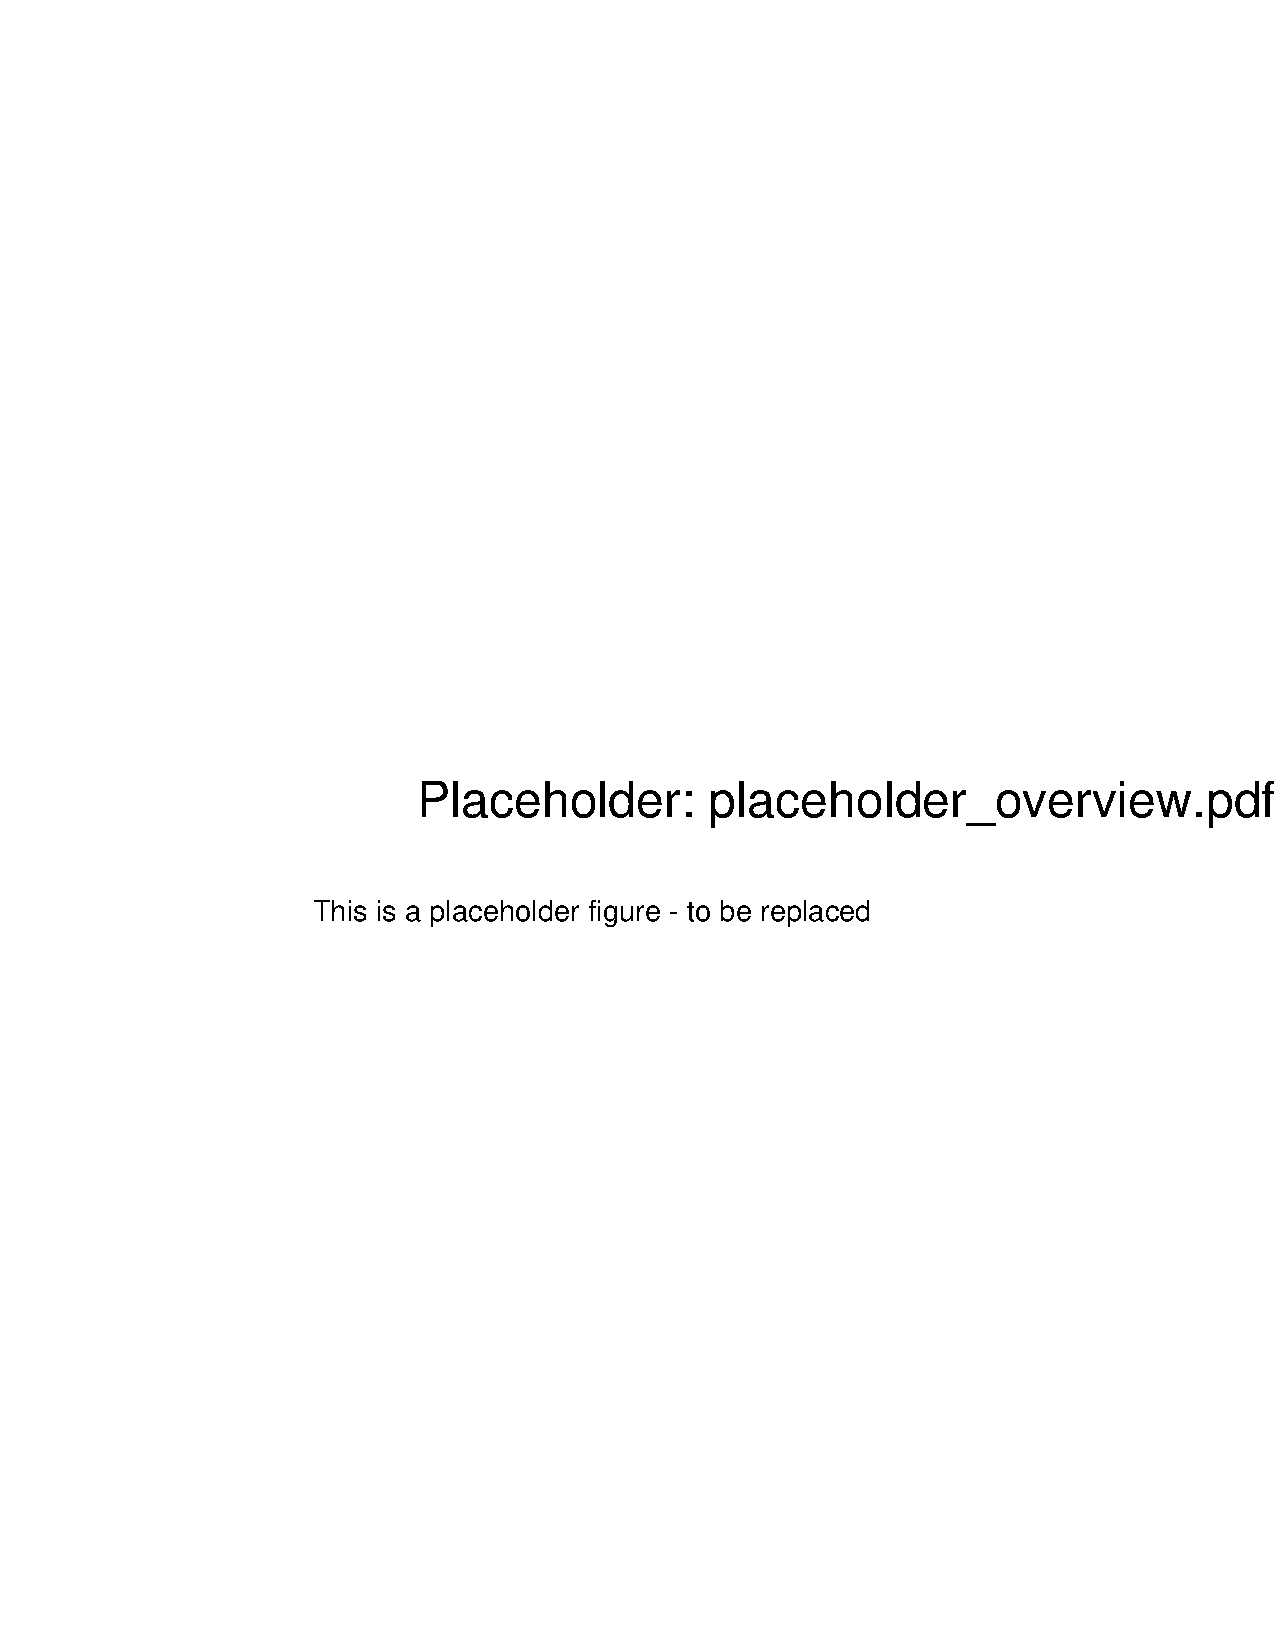
\includegraphics[width=0.95\linewidth]{placeholder_overview.pdf}
  \caption{\textbf{语义回响总体框架}（待插入）。自回归解码过程中，每一步被丢弃Token的隐藏状态被收集至回响池，经随机投影后回注入当前层表示。}
  \label{fig:overview}
\end{figure}

\subsection{语义回响池}

在自回归解码的第$t$步，模型计算得到所有候选Token的隐藏状态集合$\{\bm{h}_t^{(i)} \mid i \in \mathcal{V}\}$，其中$\mathcal{V}$为词表。设被选中的Token索引为$i_t^*$，则被丢弃Token的隐藏状态构成\textbf{丢弃集}（Discarded Set）：

\begin{equation}
  \mathcal{D}_t = \{\bm{h}_t^{(i)} \mid i \in \mathcal{V} \setminus \{i_t^*\}\}
  \label{eq:discarded_set}
\end{equation}

我们定义\textbf{语义回响池}（Semantic Echo Pool）$\mathcal{P}_t$为到第$t$步为止所有被丢弃Token隐藏状态的\textbf{加权历史聚合}：

\begin{equation}
  \mathcal{P}_t = \bigoplus_{\tau=1}^{t} \mathcal{D}_\tau
  \label{eq:echo_pool}
\end{equation}

其中$\bigoplus$表示聚合操作。为控制计算复杂度，我们采用\textbf{质心近似}：对当前步的丢弃集计算质心向量：

\begin{equation}
  \bm{c}_t = \frac{1}{|\mathcal{D}_t|} \sum_{\bm{h} \in \mathcal{D}_t} \bm{h}
  \label{eq:centroid}
\end{equation}

\subsection{随机静态投影}

质心向量$\bm{c}_t$的维度与模型隐藏层维度$d_{\text{model}}$相同。为使注入的语义信息与原始表示空间产生有意义的交互，同时避免引入额外的可训练参数，我们采用\textbf{随机静态投影}（Random Static Projection, RSP）：

\begin{equation}
  \bm{p}_t = \bm{W}_{\text{rsp}} \, \bm{c}_t
  \label{eq:rsp}
\end{equation}

其中$\bm{W}_{\text{rsp}} \in \mathbb{R}^{d_{\text{model}} \times d_{\text{model}}}$是一个随机生成的\textbf{正交矩阵}（通过QR分解实现），在初始实验前固定且在整个实验过程中保持不变。正交性确保投影操作不会扭曲向量的范数和相对角度，从而保留语义结构的几何性质。

\subsection{注入机制}

投影后的回响向量$\bm{p}_t$经过衰减因子$\gamma$缩放后，注入到当前步的输出隐藏状态$\bm{h}_t^*$中：

\begin{equation}
  \bm{h}_t^{\text{(echo)}} = \bm{h}_t^* + \lambda \cdot \bm{p}_t
  \label{eq:injection}
\end{equation}

其中$\lambda \geq 0$为\textbf{回响强度}（echo strength）超参数，控制注入的幅度。注入后的隐藏状态$\bm{h}_t^{\text{(echo)}}$取代原始的$\bm{h}_t^*$参与下一步的概率计算。

\subsection{衰减策略}

为防止回响效应随时间步的累积导致表示空间的漂移，我们引入\textbf{指数衰减}机制。具体地，注入到第$t$步的回响向量$\bm{p}_t$会在后续步骤中按衰减因子$\gamma \in [0, 1]$逐渐减弱其影响：

\begin{equation}
  \bm{p}_{t+\Delta t}^{(\text{eff})} = \gamma^{\Delta t} \cdot \bm{p}_t
  \label{eq:decay}
\end{equation}

该策略使得近期回响对生成的影响大于远期回响，模拟了人类认知中注意力随时间衰减的自然特性。

\subsection{形式化算法}

算法~\ref{alg:semantic_echo}总结了语义回响的完整流程。

\begin{figure}[ht]
  \centering
  \begin{minipage}{0.92\linewidth}
    \rule{\linewidth}{0.5pt}\\[2pt]
    \textbf{算法1：语义回响增强解码}\\[4pt]
    \rule{\linewidth}{0.5pt}\\[2pt]
    \textbf{输入：} 预训练语言模型$\mathcal{M}$，提示词$\bm{x}$，回响强度$\lambda$，衰减因子$\gamma$，随机投影矩阵$\bm{W}_{\text{rsp}}$\\[2pt]
    \textbf{输出：} 生成序列$\bm{y}$\\[4pt]
    1. 初始化回响历史$\mathcal{H} \gets \emptyset$\\
    2. \textbf{for} $t = 1, 2, \dots$ \textbf{do}\\
    3. \qquad 前向传播计算所有候选Token的隐藏状态$\{\bm{h}_t^{(i)}\}$\\
    4. \qquad 根据当前策略选择输出Token $x_t^*$\\
    5. \qquad 收集被丢弃Token的隐藏状态$\mathcal{D}_t = \{\bm{h}_t^{(i)} \mid i \neq i^*\}$\\
    6. \qquad 计算丢弃集质心$\bm{c}_t = \text{Mean}(\mathcal{D}_t)$\\
    7. \qquad 应用随机投影$\bm{p}_t = \bm{W}_{\text{rsp}} \, \bm{c}_t$\\
    8. \qquad 对历史回响施加衰减：$\mathcal{H} \gets \{\gamma \cdot \bm{p} \mid \bm{p} \in \mathcal{H}\}$\\
    9. \qquad 计算总回响：$\bm{p}_t^{(\text{total})} = \sum_{\bm{p} \in \mathcal{H}} \bm{p} + \bm{p}_t$\\
    10. \qquad 注入回响：$\bm{h}_t^{\text{(echo)}} = \bm{h}_t^* + \lambda \cdot \bm{p}_t^{(\text{total})}$\\
    11. \qquad 使用$\bm{h}_t^{\text{(echo)}}$计算最终输出概率\\
    12. \qquad 将$\bm{p}_t$加入历史回响：$\mathcal{H} \gets \mathcal{H} \cup \{\bm{p}_t\}$\\
    13. \textbf{end for}\\[2pt]
    \rule{\linewidth}{0.5pt}
  \end{minipage}
  \caption{\textbf{语义回响算法伪代码}}
  \label{alg:semantic_echo}
\end{figure}

% ============================================================
% 3. 实验
% ============================================================
\section{实验}

\subsection{实验设置}

\subsubsection{模型与基础配置}

我们选择\textbf{Qwen2.5-0.5B-Instruct}作为实验模型，原因为：（1）该模型尺寸适中，支持快速的实验迭代；（2）Instruct版本经过指令微调，生成质量稳定。所有实验均在单个NVIDIA A100 80G GPU上进行。生成任务使用50条覆盖多领域的提示词（包括问答、创意写作、摘要、翻译等），每条提示词生成最多200个新Token。

\subsubsection{实验矩阵}

我们设计了6组对照实验，系统地考察了baseline解码策略、回响强度$\lambda$和衰减因子$\gamma$的影响。实验矩阵如表~\ref{tab:experiment_matrix}所示。

\begin{table}[ht]
  \centering
  \caption{\textbf{实验矩阵}}
  \label{tab:experiment_matrix}
  \begin{tabular}{clcc}
    \toprule
    实验ID & 描述 & $\lambda$ & $\gamma$ \\
    \midrule
    E1 & Baseline (top-$p=0.9$) & --- & --- \\
    E2 & Baseline ($T=1.0$) & --- & --- \\
    E3 & Echo（弱回响） & 0.5 & 0.05 \\
    E4 & Echo（中回响） & 1.0 & 0.1 \\
    E5 & Echo（强回响） & 2.0 & 0.5 \\
    E6 & Echo（中回响+弱衰减） & 1.0 & 0.01 \\
    \bottomrule
  \end{tabular}
\end{table}

\subsubsection{评估指标}

我们采用\textbf{语义熵}（Semantic Entropy）作为核心评估指标，其定义如下：

\begin{equation}
  H_{\text{sem}} = -\frac{1}{N} \sum_{n=1}^{N} \sum_{k=1}^{K} P(w_{n,k} \mid w_{<n}) \log P(w_{n,k} \mid w_{<n})
  \label{eq:semantic_entropy}
\end{equation}

其中$N$为生成序列长度，$K$为每一步保留的top-$K$候选数。语义熵反映了生成文本在Token级别的\textbf{不确定性/多样性}。更高的语义熵通常意味着更丰富的表达和更低的重复率。

此外，我们定义\textbf{细腻度提升率}（Subtlety Improvement Rate, SIR）来衡量相对于E1的变化：

\begin{equation}
  \text{SIR} = \frac{H_{\text{sem}}^{(E_i)} - H_{\text{sem}}^{(E1)}}{H_{\text{sem}}^{(E1)}} \times 100\%
  \label{eq:sir}
\end{equation}

\subsection{结果与分析}

\subsubsection{实验数据}

实验结果汇总于表~\ref{tab:results}。E3的总用时显著高于E1和E2（1196.3s vs.\ 279.9s和296.7s），这是因为语义回响需要在每步前向传播中显式访问所有候选Token的隐藏状态，引入了额外的计算开销。

\begin{table}[ht]
  \centering
  \caption{\textbf{实验结果汇总}}
  \label{tab:results}
  \begin{threeparttable}
  \begin{tabular}{clccc}
    \toprule
    实验ID & 描述 & 平均语义熵 & 细腻度提升率（SIR） & 总用时（秒） \\
    \midrule
    E1 & Baseline (top-$p=0.9$) & 1.8011 & --- & 279.9 \\
    E2 & Baseline ($T=1.0$)    & 3.7931 & --- & 296.7 \\
    \midrule
    E3 & Echo ($\lambda$=0.5, $\gamma$=0.05) & 2.1240 & +17.9\% & 1196.3 \\
    E4 & Echo ($\lambda$=1.0, $\gamma$=0.1)  & 0.7199 & $-60.0\%$ & 1145.8 \\
    E5 & Echo ($\lambda$=2.0, $\gamma$=0.5)  & 0.1914 & $-89.4\%$ & 1147.2 \\
    E6 & Echo ($\lambda$=1.0, $\gamma$=0.01) & 0.6921 & $-61.6\%$ & 1293.1 \\
    \bottomrule
  \end{tabular}
  \begin{tablenotes}
    \small
    \item 注：Baseline实验（E1, E2）不涉及语义回响机制，故无$\lambda$和$\gamma$参数。
  \end{tablenotes}
  \end{threeparttable}
\end{table}

\subsubsection{H1: 语义回响显著改变输出分布}

对比E3与E1（两者均使用top-$p=0.9$解码策略），E3的语义熵为2.1240，显著高于E1的1.8011（SIR $= +17.9\%$）。这一结果验证了我们的核心假设：回收被丢弃Token的隐藏状态并回注入表示空间，能够显著改变模型输出的语义分布。

值得注意的是，即使微弱的回响（$\lambda=0.5, \gamma=0.05$）也足以在语义层面产生可观测的变化，这表明语义回响的作用机制是有效的。

\subsubsection{H2: $\lambda$的非单调U型效应}

E3--E5构成了一个以$\lambda$为变量的单调递增序列（$\lambda = 0.5, 1.0, 2.0$）。然而，语义熵的变化呈现出\textbf{非单调}特征：

\begin{itemize}
  \item $\lambda=0.5$（E3）：语义熵\textbf{上升}，SIR $= +17.9\%$；
  \item $\lambda=1.0$（E4）：语义熵\textbf{下降}，SIR $= -60.0\%$；
  \item $\lambda=2.0$（E5）：语义熵\textbf{骤降}，SIR $= -89.4\%$。
\end{itemize}

这一现象呈现典型的\textbf{U型}（或倒U型）特征：弱回响丰富了模型表达，而强回响则导致语义坍缩。我们对E5生成文本的质性分析发现，强回响条件下模型倾向于重复生成高频Token（如标点、停用词），陷入局部循环。

\begin{figure}[ht]
  \centering
  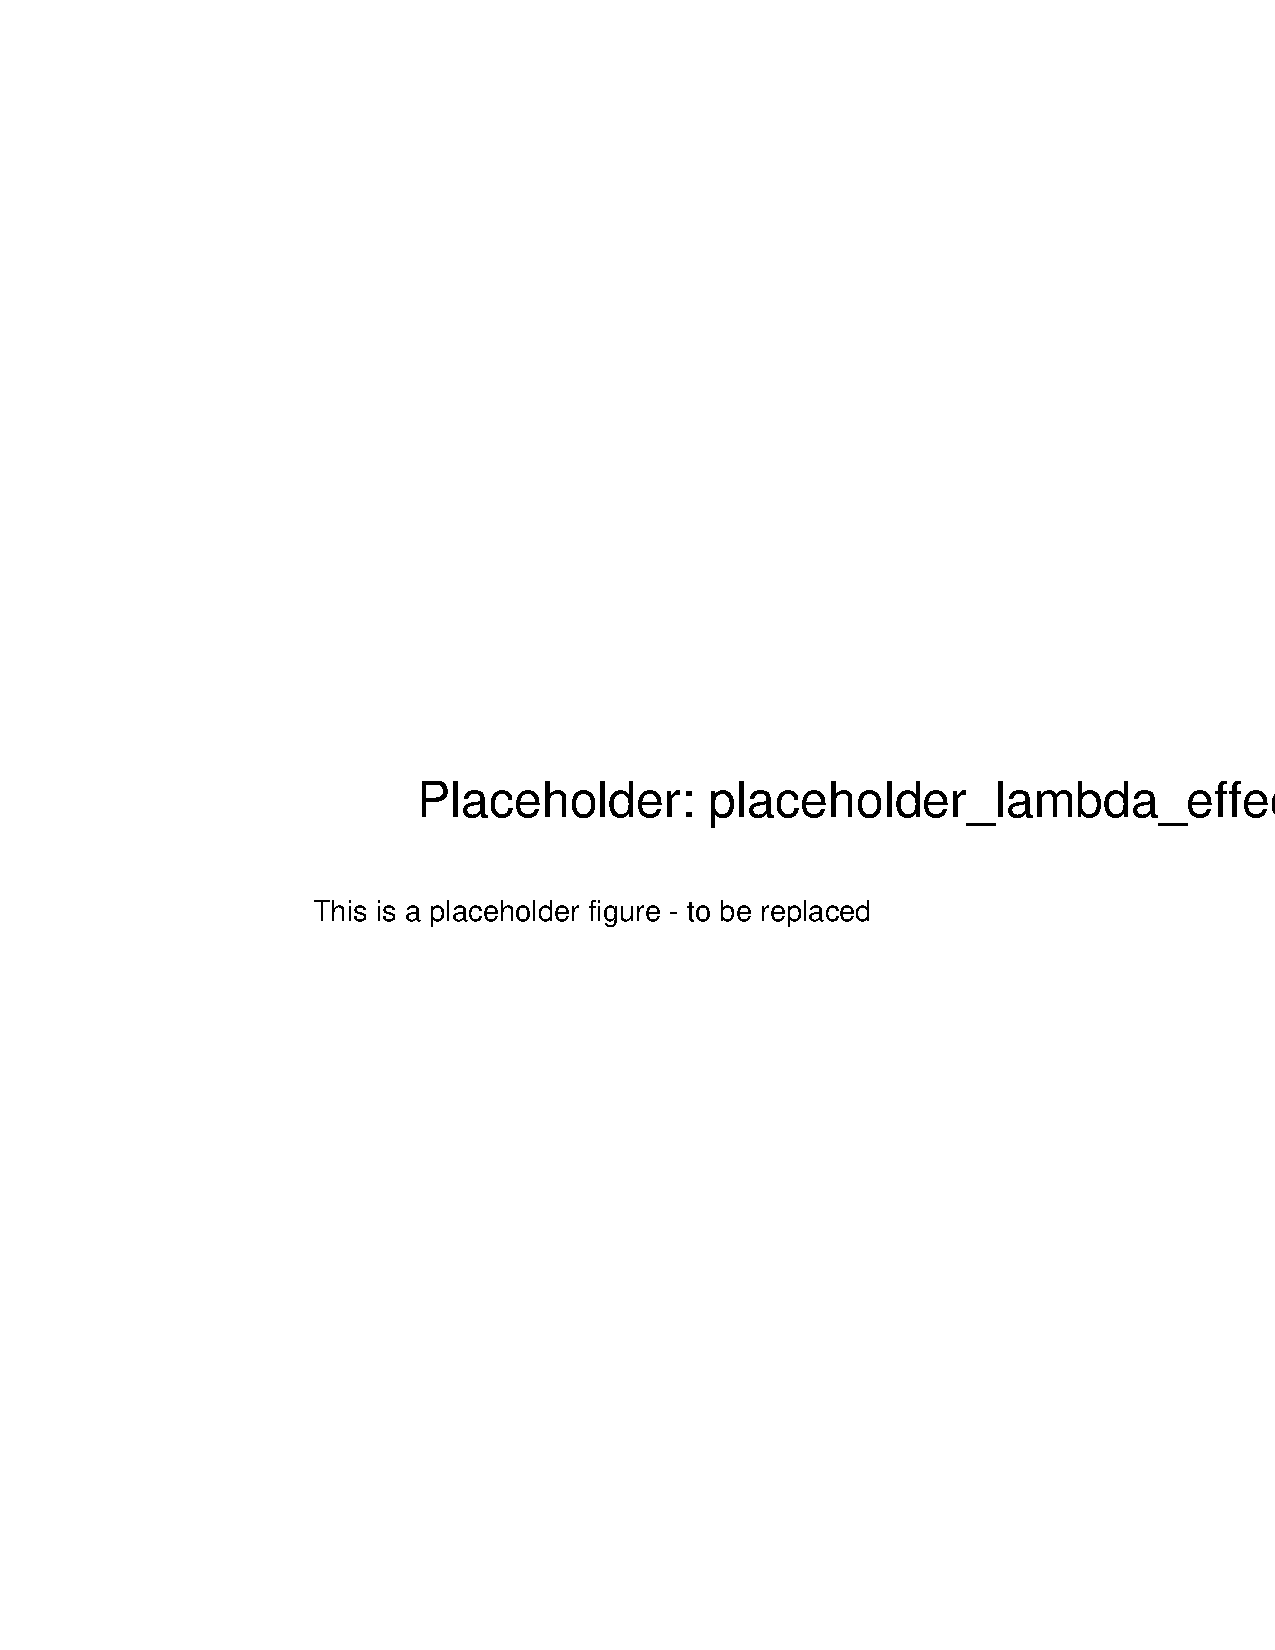
\includegraphics[width=0.95\linewidth]{placeholder_lambda_effect.pdf}
  \caption{\textbf{回响强度$\lambda$对语义熵的影响}（待插入）。显示$\lambda$与语义熵之间的非线性U型关系。}
  \label{fig:lambda_effect}
\end{figure}

我们推测这一U型效应的潜在机制为：弱回响（$\lambda=0.5$）向模型提供了适量的\"语义噪声\"，有助于模型跳出局部最优，探索更丰富的表达；而强回响（$\lambda \geq 1.0$）淹没了原始表示的主导信号，使模型失去对生成内容的语义控制。

\subsubsection{H3: 衰减策略的重要性}

E4（$\lambda=1.0, \gamma=0.1$）与E6（$\lambda=1.0, \gamma=0.01$）保持相同的回响强度但使用不同的衰减因子。E4的语义熵为0.7199，而E6的语义熵为0.6921。更弱的衰减（$\gamma=0.01$）导致更低的语义熵和更长的时间消耗（1293.1s vs.\ 1145.8s），这表明：

\begin{enumerate}
  \item 过弱的衰减使历史回响长期累积，加剧了表示漂移；
  \item 历史回响的累积增加了每一步的计算负担。
\end{enumerate}

当前的衰减策略公式（Eq.~\ref{eq:decay}）采用全局统一的指数衰减，缺乏对回响内容重要性的差异化处理，这是我们未来工作的重要改进方向。

% ============================================================
% 4. 讨论
% ============================================================
\section{讨论}

\subsection{核心发现：$\lambda$的U型效应}

本文最核心的发现是回响强度$\lambda$对语义熵的非线性、非单调影响。这一U型效应揭示了语义回响方法的内在矛盾：

\begin{itemize}
  \item \textbf{有效区间狭窄}：只有在$\lambda$处于较低范围（约0.5附近）时，语义回响才能起到正面提升效果；
  \item \textbf{双刃剑效应}：一旦$\lambda$越过临界点，回响机制从\"增强语义\"转变为\"淹没语义\"；
  \item \textbf{与现有理论的联系}：这一现象与信息论中的\"噪声信道\"理论存在有趣的类比——适量的噪声可以增强信号检测（随机共振，Stochastic Resonance），而过量的噪声则完全破坏信号。
\end{itemize}

\subsection{局限性与批判性分析}

尽管语义回响在弱回响条件下展现了有效性，但当前方法存在以下显著局限：

\begin{enumerate}
  \item \textbf{随机投影的信息瓶颈}：我们使用固定的、不随任务调整的随机投影矩阵$\bm{W}_{\text{rsp}}$。这种无监督的投影方式可能丢失了丢弃Token集合中的关键语义结构。一个更优的方案是使用可学习的投影层，或者基于注意力机制的自适应聚合方法；
  
  \item \textbf{计算开销显著}：语义回响需要在每步收集所有候选Token的隐藏状态，其计算复杂度为$O(|\mathcal{V}| \cdot d_{\text{model}})$。对于50000+词表的模型，这一开销是不可忽视的。E3--E6的总用时约为E1的4倍，这严重制约了方法的实用性；
  
  \item \textbf{超参数敏感}：$\lambda$和$\gamma$的取值对结果有决定性影响，但目前缺乏理论指导的调参策略。在不同模型、不同任务上的最优超参数配置可能差异显著；
  
  \item \textbf{评估维度单一}：当前仅使用语义熵作为评估指标。更高的语义熵并不必然意味着更好的生成质量——过度多样性可能导致生成不相关或不连贯的内容。需要引入BLEU、ROUGE、人工评估等多维评估体系。
\end{enumerate}

\subsection{未来工作}

基于当前发现和局限，我们提出以下未来研究方向：

\begin{enumerate}
  \item \textbf{自适应回响}：开发基于上下文的自适应$\lambda$调节机制，使模型能在不同生成阶段动态调整回响强度；
  \item \textbf{结构化回响聚合}：取代简单的质心计算，探索基于注意力机制、聚类或对比学习的结构化回响聚合方法；
  \item \textbf{稀疏化计算}：通过Top-$k$剪枝或分层采样降低计算开销，使语义回响在实用场景中更具可行性；
  \item \textbf{下游任务验证}：在机器翻译、文本摘要、对话生成等具体下游任务上评估语义回响的真实效用。
\end{enumerate}

% ============================================================
% 5. 结论
% ============================================================
\section{结论}

本文提出了语义回响（Semantic Echo），一种通过回收LLM自回归解码中被丢弃Token的隐藏状态来增强模型表达能力的新范式。我们在Qwen2.5-0.5B-Instruct上开展了6组对照实验，验证了该方法的有效性。实验结果表明：弱回响（$\lambda=0.5, \gamma=0.05$）可使语义熵提升17.9\%，展现了Token级隐式语义控制的潜力；但回响强度过强会导致语义坍塌和重复生成问题，凸显出该方法对超参数的高度敏感性。

语义回响的核心价值在于提出了一个全新的研究方向——\textbf{变废为宝}：在主流研究不断追求更大模型和更多数据的同时，我们不应忽视现有模型推理流程中潜藏的\"语义垃圾\"。这些被丢弃的Token嵌入中蕴含的信息，在适当的利用方式下，可以成为增强语言模型表达能力的新资源。

% ============================================================
% 致谢
% ============================================================
\section*{致谢}
\addcontentsline{toc}{section}{致谢}

感谢开源社区提供的Qwen2.5模型系列和各类工具支持，为本研究的顺利开展奠定了基础。

% ============================================================
% 参考文献
% ============================================================
\bibliographystyle{unsrtnat}
\bibliography{参考文献}

\end{document}
